
\documentclass[conference]{IEEEtran}
%





% *** GRAPHICS RELATED PACKAGES ***

\usepackage[english]{babel}
\usepackage[utf8]{inputenc}
\usepackage{graphicx}
\usepackage{algorithm}
\usepackage[noend]{algpseudocode}
\usepackage{tikz}
\usetikzlibrary{shapes,positioning,matrix}
\usepackage{amsmath}

\DeclareMathOperator{\dis}{d}

%
\ifCLASSINFOpdf
  
\else
  
\fi



\begin{document}

\title{Self-Trainable 3D Printed Prosthetic Hand Customized Control System Architecture with SVM Classification by using EMG Signals}

\author{\IEEEauthorblockN{Kyungho Nam}
\IEEEauthorblockA{Department of Computer Science\\
Oklahoma State University\\
Stillwater, OK 74078\\
kyungho.nam@okstate.edu}
\and
\IEEEauthorblockN{Christopher Crick}
\IEEEauthorblockA{Department of Computer Science\\
Oklahoma State University\\
Stillwater, OK 74078\\
chriscrick@cs.okstate.edu}}


% make the title area
\maketitle

%%% ABSTRACT
\begin{abstract}
The United Nations published the Convention on the Rights of Persons with Disabilities, which promotes that persons with disabilities have the right to receive the highest quality and standard of free or affordable health care \cite{UN}. However, the World Health Organization has recorded that only 5-15\% people can reachable adequate prosthesis service \cite{WHO}. This paper provides an overview of self-trainable user-customized system architecture for a 3D printed prosthetic hand to reduce the challenge of accessing and maintaining these supporting devices. In this paper, developing and implementing a customized behavior system can generate any gesture that users desire. This system architecture interacts and communicates with electromyography with MyoWare Muscle Sensor between the user's arm and 3D printed prosthetic hand.
\end{abstract}

% Note that keywords are not normally used for peer review papers.
\begin{IEEEkeywords}
EMG, prosthetic hand, Self-trainable, SVM, RBF.
\end{IEEEkeywords}


\IEEEpeerreviewmaketitle


%%% INTRODUCTION
\section{Introduction}
\IEEEPARstart{A}{ccording} to the General Assembly from United Nations, Article 25 of Convention on the Rights of Persons with Disabilities which is the resolution adopted by the General Assembly mentioned that the right to receive the highest feasible standard of health without discrimination on the basis of disability from States Parties \cite{UN}. For implementing this to the amputee, the provision of affordable and high-quality prosthetic aids can be a human rights argument, one that the government must support. Nevertheless, World Health Organisation figures that only 5-15\%, which is approximately 1 in 10 people of the population in need, is able to access prosthetic and orthotic appliances in today's world \cite{WHO}. The difficulty of accessing such devices is more important in low- and middle-income countries. In this area, charities with non-trained professionals often provide prosthetic and orthotic services meaning that service quality is compromised, which results in poor quality and fit. Without adequate maintenance service access to prosthetic and orthotic services, people are often restricted to their quality of life, excluded from participating in society, and locked into poverty and isolation \cite{WHO}.

The weighted average prosthesis price is \$10,232, and total costs for the prosthesis after second year are \$181,500 \cite{cost}. The annual maintenance costs for the prosthesis are expected to be 20\% of the prosthesis' price, for a total of \$83,490 after second year \cite{cost}.

To fulfill the necessity of excellent quality maintenance service and to resolve the lack of high performing prosthesis because of the high cost, this paper introduces an architecture that can be self-trainable and user-customized 3D printed prosthetic hand. This architecture provides self-trainable software to the user, which can increase the prosthetic hand's performance with \$0 financial cost. A small amount of time investing in training the user's prosthesis returns high accuracy in its performance with repetitive behavior through this system.




\section{Related Work and Contributions}
\subsection{3D Printed Prosthesis}
There are many efforts and studies, which have been conducted so that more people can use low-cost prosthetics. Many of the prior research started to focus on the trial to make prosthetics with 3d printers to satisfy users' financial needs. Several recent works \cite{3D2}\cite{3D4} aimed to build a low cost robotic prosthetic arm on the use of 3D printing technology with capable and comfortable design. 3D printing technology suggests a new path to sufficient amputees' financial needs and various physical conditions with departing from the prosthesis's standard size for children or veterans with upper limb loss. \cite{3D3} The research \cite{3D1} developed a hand prototype using the same structure of a human hand with using 5 servo motors and electromyography (EMG) sensors to detect the electrical potential when muscle contraction appears, which became the foundation for the prototype of this architecture. 

\subsection{Action Classification}
To enhance the performance of the imagined hand movement using the non-invasive control technique, Brain-Machine Interface (BMI) research used the electroencephalogram (EEG). \cite{EEG}. The features were extracted using RBF kernel SVM classifier \cite{ML1}\cite{ML2}, achieved 92.75\% for the average accuracy compared to 81.12\% obtained with Linear SVM classifier. \cite{EEG} 


Based on these researches, the problem we consider was the customization for each diverse users. The perfectly fitting prosthesis with high performance for all the different individuals is impracticable.

In our approach, this developed architecture can users train their devices not only smarter with high performance but also creative with any kinds of new behavior the user wants.


\section{Control System Architecture Components}
In this section we provide a detailed description of the individual control system components of this architecture.




\subsection{3D Printed Prosthetic Hand}
Many of the open-source prosthetic hands' floor print is available. All the prosthesis parts are into stereolithography (STL) files with different designs that are possible to be modified for the best fittable model for each different user. With those STL files, the 3D printer printed the prosthetic hand with different diverse sizes for different people who need it. For the experiments, an open-source design was adopted and printed with a 3D printer, which is easily modified in the future for each user's needs.


In this prosthesis prototype, 5 servo motors were used for the actuator. Each servo motor mg996r is connected with each finger. The mg996r motors were controlled by an Arduino Mega microcontroller, which is the board consist of an Atmel 8-bit AVR microcontroller. When the EMG sensors detect a muscle contraction, the microcontroller controls individual servo motors to control individual fingers in real-time through the decision-making process. The printed 3D prosthetic hand is shown in Fig. \ref{hand}.

\begin{figure}[h]
  \centering
  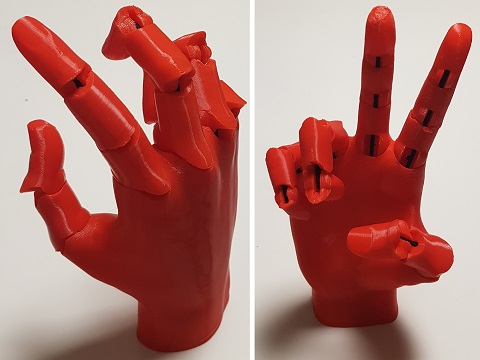
\includegraphics[width=3.4in]{3dhand3.jpg}
  \caption{3D printed prosthetic hand}
  \label{hand}
\end{figure}


%% Electromyography Signal
\subsection{Electromyography Signal}

\subsubsection{EMG Sensors}

To detect and measure muscle contraction, produced electrical activity, the electrodiagnostic technique is considered as an input for the decision-making process. The MyoWare Muscle Sensor is used, which is designed by microcontroller applications \cite{myo} with the dimension of 52.3x20.7mm, which needs a voltage power between 2.9-5.7 V with a maximum current of 14mA. As shown in Fig. \ref{myo}, the sensor can measure the muscle's electrical potential with three electrodes when the sensor board is placed at the skin above the targeted muscle.

\begin{figure}[h]
  \centering
  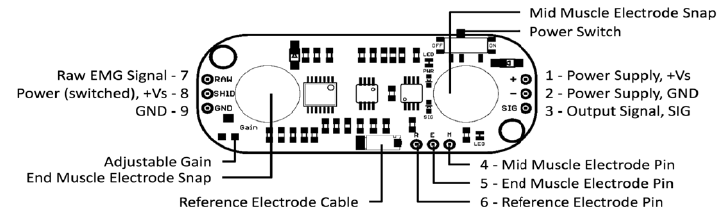
\includegraphics[width=3.4in]{myosensor.png}
  \caption{The layout of the MyoWare Muscle Sensor (AT-04-001)}
  \label{myo}
\end{figure}


\subsubsection{EMG Signal Processing}

The MyoWare Sensor can detect envelope EMG and raw EMG with the voltage signal difference between the central muscle electrode and the reference electrode. The sensor generates the envelope signal, which is amplified, rectified, and integrated within the sensor transducer, as shown in Fig. \ref{signal}. The signal amplitude is utilized to features to decide a human behavior at the decision-making process with a microcontroller's analog-to-diginal converter (ADC).

\begin{figure}[h]
  \centering
  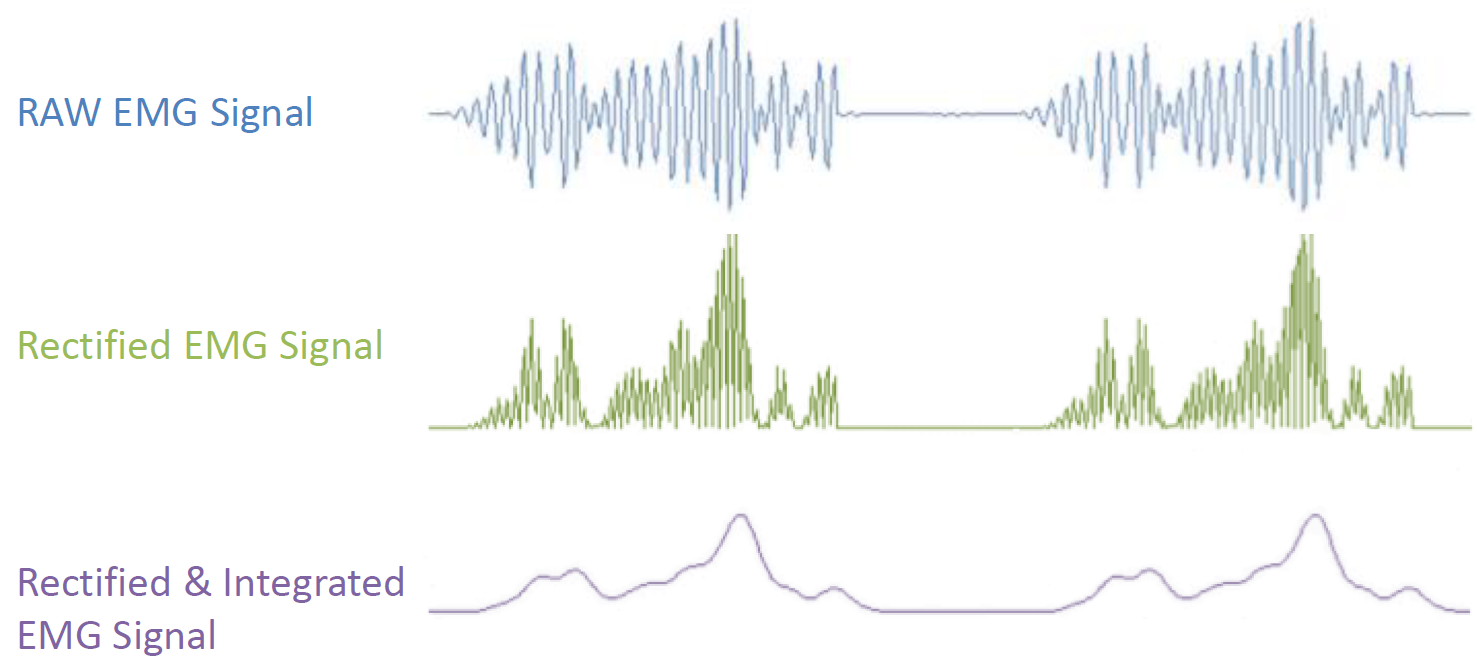
\includegraphics[width=3.4in]{signals.png}
  \caption{An example of the EMG signals processing}
  \label{signal}
\end{figure}


\subsection{Self Training User Customize Control Software}

In our software designed to train the user's prosthetic hand, all the magnitude of the envelope signals, generated by 3 channel EMG sensor signals, were transferred to the Arduino platform. The microcontroller can read and record all the sensor data as a user history to train each behavior into the machine. In the trained device, those 3 matrix values contain 0 to 1000 magnitude sensor value as inputs are the factors of prosthetic hand behavior decision-making in real-time.
The training function procedure and the actual operate function procedure system algorithm is listed in Algorithm 1.

% Algorithm
\begin{algorithm}
\caption{System Architecture}
\label{alg:sysArch}
\begin{algorithmic}[1]
\Procedure{Training}{}

\State \textit{y.append(CustomGesture)}
\Comment{custom new gesture}
\For {$i=y_{0}$ to $y_{max}$}
    \For {$j=0$:$T$}
        \State $ \textit{$X_{j}^i$} \gets \textit{readSensors()}$
        \EndFor
    \EndFor
\State \textit{clf.fit(X, y)}
\EndProcedure

\Procedure{Movements}{}
\While{$r\not=0$}
\State \textit{ $Gesture = predict(readSensors()) $}
\State \textit{ $MotorController(Gesture, servoMotors())$ }
\EndWhile\label{endwhile}
\EndProcedure
\end{algorithmic}
\end{algorithm}

Support vector machines (SVMs) \cite{ML1}\cite{ML2} of supervised learning methods is applied to the prosthetic hand's behavior classification. This gesture classification used multiple EMG sensors as input matrix X, and the output matrix y consists of each different individual intended gestures.  

The equation \eqref{kernel} defines the radial basis function kernel for two different inputs X and X', designated as feature vectors, which is the factor to predict purposing action with trainable high-performance accuracy.
\begin{equation}
K(X,X') = \exp(-\frac{\lVert X - X' \rVert^2}{2\sigma^2})
\label{kernel}
\end{equation}

The squared Euclidean distance between the two feature vectors is shown in $\lVert X - X' \rVert^2$.
The $\sigma$ worked as a parameter condition.

The artificial neural network interpretation of SVMs using radial basis function kernel to train the prosthesis is demonstrated in Fig. \ref{RBF}.

%% RBF figure
\begin{figure}[htp]
\centering
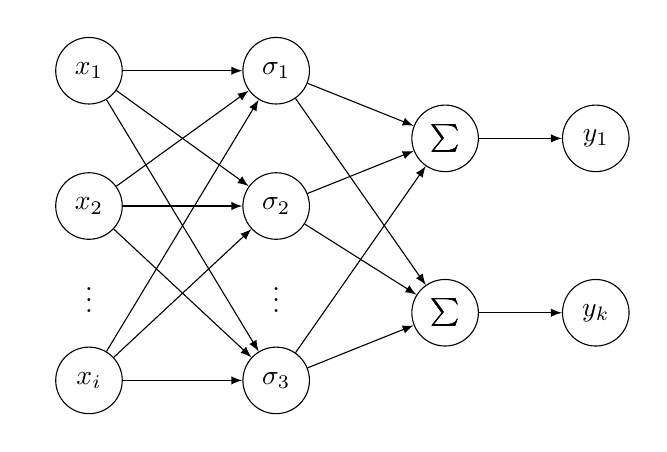
\begin{tikzpicture}[
plain/.style={
  draw=none,
  fill=none,
  },
net/.style={
  matrix of nodes,
  nodes={
    draw,
    circle,
    inner sep=8.5pt
    },
  nodes in empty cells,
  column sep=0.6cm,
  row sep=-11pt
  },
>=latex
]
\matrix[net,row sep=0em, column sep=3em] (mat)
{
             &           \\
  |[plain]|  & |[plain]| &  &         \\
             &           \\
  |[plain]|$\vdots$ & |[plain]|$\vdots$ &  &       \\
             &           \\
};
\foreach \ai in {1,3,5}
  {\foreach \aii in {1,3,5}
    \draw[->] (mat-\ai-1) -- (mat-\aii-2);
}
\foreach \ai in {1,3,5}
  {\foreach \aii in {2,4}
    \draw[->] (mat-\ai-2) -- (mat-\aii-3)node(){$\sum$};
}
\draw[->] (mat-2-3) -- (mat-2-4)node(){$y_1$};
%\draw[->] (mat-2-5)node(){$t_i$} -- (mat-2-4);
 
\draw[->] (mat-4-3) -- (mat-4-4)node(){$y_k$};
% \draw[->] (mat-4-5)node(){$t_k$} -- (mat-4-4);

\node(x1) at (mat-1-1){$x_1$}; \node(s1) at (mat-1-2){$\sigma_1$};
\node(x1) at (mat-3-1){$x_2$}; \node(s2) at (mat-3-2){$\sigma_2$};
\node(x1) at (mat-5-1){$x_i$}; \node(s3) at (mat-5-2){$\sigma_3$};
\end{tikzpicture}
\caption{Radial basis function model}
\label{RBF}

\end{figure}

The support vector classification implementation is tuned regularization parameter C = 2.5, and the kernel coefficient for RBF gamma = 0.01.




%%% Experimentation and Results`
\section{Experimentation and Results}
The subject in the experiment is instructed to attach three EMG muscle sensors to the subject's muscles which shown in Fig \ref{pic}.

\begin{figure}[h]
  \centering
  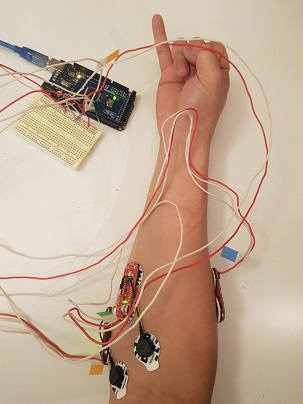
\includegraphics[width=2.7in]{am.jpg}
  \caption{User's unique gesture (Pinky Swear) training with 3 EMG sensors}
  \label{pic}
\end{figure}

The EMG muscle sensors are attached on the area of flexor digitorum superficialis, which is an extrinsic flexor muscle to actuate four fingers with the interphalangeal joints, flexor digitorum profundus, which is the muscle that can bend the fingers to grip, and flexor pollicis longus, which actuates thumbs, particularly for writing and painting.

To train various gestures into the prosthetic hand, a trial of using the prosthetic hand with 3 EMG MyoWare Muscle Sensors is performed. The subject tried to contract his muscles to behave his intended hand actions and retained for a while. Simultaneously, EMG sensor data recorded 200 times per each action.

To testify to the decision-making algorithm's practicality, the numerous experiment routine is conducted with the EMG signals used to classify each different hand movements.


Each gesture is repeated, and simultaneously the 200 EMG muscle sensor values are recorded when the user retains his motion as shown in Table 1.

\begin{table}[ht]
\caption{Experiments with different actions} % title of Table
\centering % used for centering table
\begin{tabular}{c c} % centered columns (3 columns)
\hline\hline %inserts double horizontal lines
User behavior & Each iteration \\ [0.5ex] % inserts table
%heading
\hline % inserts single horizontal line
Hand Relax & 200 \\ % inserting body of the table
Clenching fist & 200 \\
Open hand & 200 \\
Thumbs up & 200 \\
Pointing somewhere & 200 \\
OK sign & 200 \\
Ball grip & 200 \\
Pencil grip & 200 \\
Smartphone grip & 200 \\
User's unique gesture whatever the user wants & 200 \\ [1ex] % [1ex] adds vertical space
\hline %inserts single line
\end{tabular}
\label{table:nonlin} % is used to refer this table in the text
\end{table}

Any user's customized unique gestures are recorded in the 'User's unique gesture whatever the user wants,' which can offer the customization applicability for each different user potentially.



Fig. \ref{3dplot} illustrated for two representative histories of each EMG sensor variables' cluster. Each color of scatters represents each different gestures as labels. Each axis of the graph shows the actual sensor variable boundary between 0 to 1000 amplitude, measured by 3 different MyoWare Muscle Sensors. 

\begin{figure}[h]
  \centering
  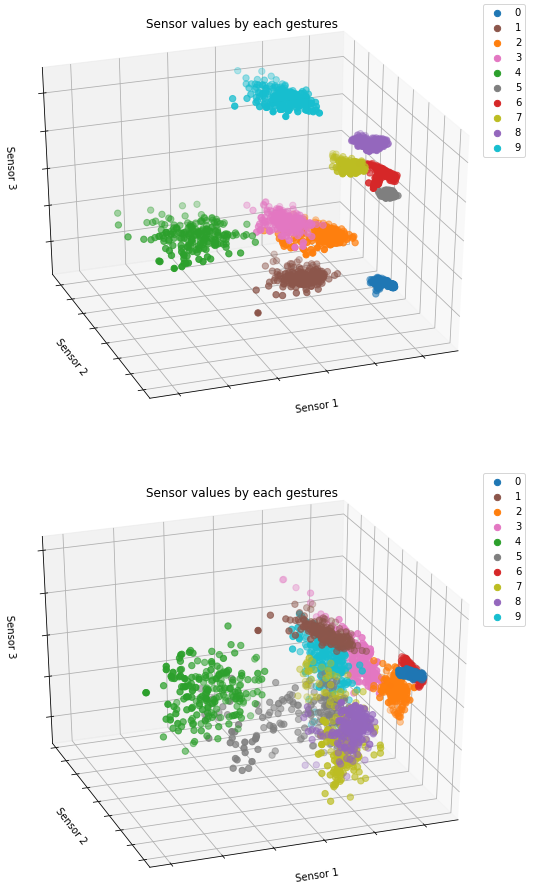
\includegraphics[width=3.4in]{pretty_f.png}
  \caption{Collected 3-channel EMG sensor values by each different action}
  \label{3dplot}
\end{figure}


The evaluation results of the model illustrated with confusion matrix as shown in Fig. \ref{cm}, which denotes the accuracy per user action label. Each column corresponds the true label, which is user's intended hand gesture, and each row corresponds the predicted label, which is the prosthetic hand actuated hand gesture.

This equation \eqref{eq} is merely equivalent to the relationship of predictions that the model classified precisely.

\begin{eqnarray}
  Accuracy & = & \frac{\textit{The number of correct predictions}}{\textit{Total number of predictions}} \\[1ex]
   & = & \frac{\textit{TP + TN}}{\textit{TP + TN + FP + FN}}
    \label{eq}
\end{eqnarray}



The train set estimated accuracy was 95.69\%, and the test set estimated accuracy was 95.50\%. As the last step of the experiment, user intended any kinds of unique gestures what he wants such as crossed fingers, V sign, finger gun, and sign of the horns, the prosthetic hand successfully working with high percentage 93\%. This result denotes applying user-customized training software into the prosthetic hand can suffice individual user requirements with high performance.

\begin{figure}[h]
  \centering
  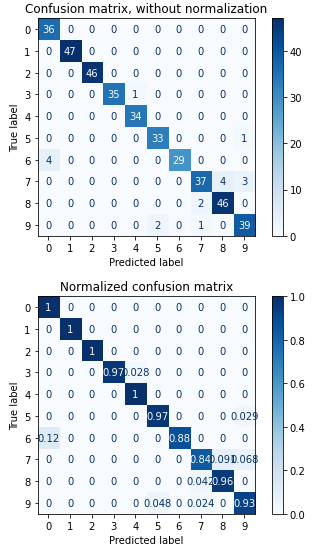
\includegraphics[width=2.5in]{confusionmatrix3.PNG}
  \caption{Confusion matrix represents the accuracy per user action label}
  \label{cm}
\end{figure}



\section{Conclusion}
This article aimed to exhibit the architecture which can provide self trainable sufficient quality of maintenance service and produce high performing prosthesis with a low economic cost. Consequently, this self-trainable customized control system for 3D printed prosthetic hand is successfully designed and tested with high performance.








% Can use something like this to put references on a page
% by themselves when using endfloat and the captionsoff option.
\ifCLASSOPTIONcaptionsoff
  \newpage
\fi



\begin{thebibliography}{1}

% \bibitem{IEEEhowto:kopka}
% H.~Kopka and P.~W. Daly, \emph{A Guide to \LaTeX}, 3rd~ed.\hskip 1em plus
%   0.5em minus 0.4em\relax Harlow, England: Addison-Wesley, 1999.

\bibitem{UN}
United Nation. \emph{Convention on the Rights of Persons with Disabilities.} 2006.

\bibitem{WHO}
World Health Organization. \emph{Standards for prosthetics and orthotics service provision: 2015–2017 work plan.} Geneva: 2015.

\bibitem{cost}
K.~C. Chung, D.~Saddawi-Konefka, S.~C. Haase, and G.~Kaul, \emph{A Cost-Utility Analysis of Amputation versus Salvage for Gustilo IIIB and IIIC Open Tibial Fractures}, Plastic and Reconstructive Surgery. 2010.

\bibitem{3D2}
N.~Sakib, J.~Pazos and M.~K. Islam, \emph{Design and Implementation of an EMG Controlled 3D Printed Prosthetic Arm}, IEEE International Conference on Biomedical Engineering, Computer and Information Technology for Health (BECITHCON). 2019.

\bibitem{3D4}
M.~Yoshikawa, R.~Sato, T.~Higashihara, T.~Ogasawara and N.~Kawashima, \emph{Rehand: Realistic electric prosthetic hand created with a 3D printer}, IEEE International Conference of the IEEE Engineering in Medicine & Biology Society (EMBC). 2015.

\bibitem{3D3}
A.~Mohammadi, J.~Lavranos, Y.~Tan, P.~Choong and D.~Oetomo, \emph{A Paediatric 3D-Printed Soft Robotic Hand Prosthesis for Children with Upper Limb Loss}, IEEE International Conference of the IEEE Engineering in Medicine & Biology Society (EMBC). 2020.

\bibitem{3D1}
A.~Cañizares, J.~Pazos and D.~Benítez, \emph{On the Use of 3D Printing Technology Towards the
Development of a Low-Cost Robotic Prosthetic Arm}, IEEE International Autumn Meeting on Power, Electronics and Computing (ROPEC). 2017.

\bibitem{EEG}
R.~Bousseta, S.~Tayeb, I.~E. Ouakouak, M.~ Gharbi, F.~Regragui and M.~M. Himmi, \emph{EEG Efficient classification of imagined hand
movement using RBF kernel SVM}, IEEE International Conference on Intelligent Systems: Theories and Applications (SITA). 2016.

\bibitem{ML1}
Bishop, Christopher M. \emph{Pattern Recognition and Machine Learning}, New York :Springer, 2006.

\bibitem{ML2}
T.~Hastie, R.~Tibshirani, and J.~H. Friedman, \emph{The elements of statistical learning: Data mining, inference, and prediction}, New York: Springer. 2001.

\bibitem{myo}
www.AdvancerTechnologies.com, \emph{MyoWare Muscle Sensor (AT-04-001) datasheet}, 2015.

\end{thebibliography}




\end{document}


